\chapter{Conception}
\label{chap:conception}
La récolte de données et la mise en place de la pipeline de traitement des données sont les éléments centrales de ce projet.
Ceux-ci peuvent être conceptualisé afin de garantir un fil rouge dans le développement de l'application.

%------------------------------------------------------------------------------
\section{Récolte des données}
Au commencement du projet, il y avait un fichier excel qui contenait les donnée de l'application.
Pour continuer à améliorer le modèle, il faut faut récupérer les nouvelles features.

\begin{center}
    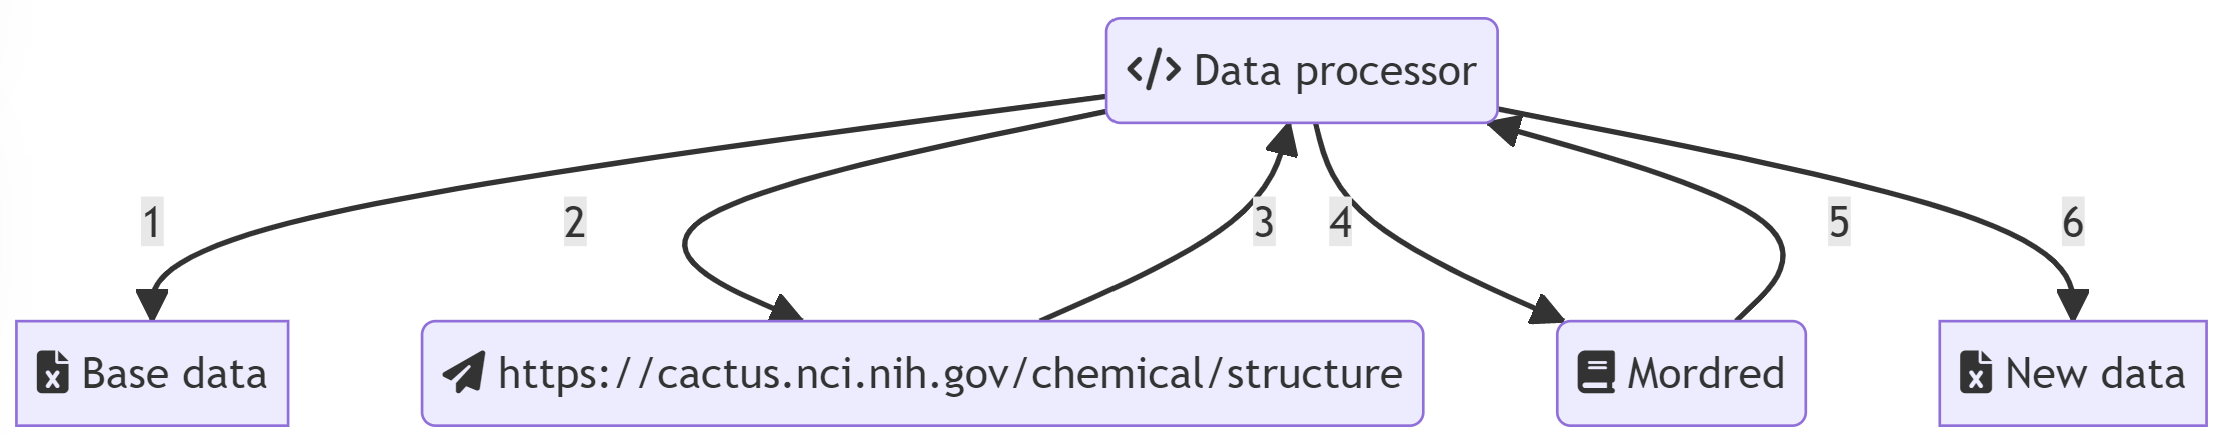
\includegraphics[width=140mm]{img/conception-data-construction.png}
    \captionof{figure}{Construction des données}
\end{center}

Le but est de prendre le nom des molécules depuis le fichiers excel existant et de traduire les noms en SMILES grâce à l'API de cactus.nci.nih.gov.
L'utilisation se fait simplement en faisant une requête HTTP GET sur l'URL suivante:
\begin{center}
    https://cactus.nci.nih.gov/chemical/structure/nomDeLaMolécule/smiles
\end{center}
Ensuite, il faut récrire les données dans un nouveau fichier excel.

Le temps de calcul des descripteurs est relativement long, il est donc intéressant de précalculer les descripteurs pour les liquides ioniques déjà présents dans le fichier excel.
Pour cela, il faut uitliser la libraire mordred\cite{mordred}.

La structure du fichier sera aussi modifiée pour faciliter la lecture des données par l'application.
Voici la structure du fichier excel de base:
\begin{itemize}
    \item IL structure: Informations des anions et cations utilisés (to test, Number, Abbreviation, Cation/Anion Full Name, Structure)
    \item Training set: Données pour l'entraînement du modèle (Cation, Anion, 99 features, Exp (K))
    \item Testing set: Données pour le test du modèle (Cation, Anion, 99 features, Exp(K))
\end{itemize}

La structure du fichier excel après la récolte des données sera:
\begin{itemize}
    \item IL structure: Informations des anions et cations utilisés (to test, Number, Abbreviation, Full Name et \acrshort{smiles})
    \item Training set: Données pour l'entraînement du modèle (\acrshort{smiles}, cation, anion et Exp (K))
    \item Testing set: Données pour le test du modèle (\acrshort{smiles}, cation, anion et Exp (K))
    \item Data descriptors: Descripteurs pré-calculés pour les liquides ioniques (\acrshort{smiles} du liquide, 900 features)
    \item Data old: Features du fichier de base (\acrshort{smiles} du liquide, 99 features)
\end{itemize}

Le fichier de base contient des feuilles qui ne sont pas détaillées ici mais elles ne sont pas utilisées dans ce projet.


% -----------------------------------------------------------------------------
\section{Pipeline de Machine Learning}
Comme pour la récolte des données, il faut aussi conceptualiser la pipeline de Machine Learning.
Dans ce cas, il y a deux use case.
Le premier est l'entraînement du modèle tandis que le second est la prédiction des données.

\begin{center}
    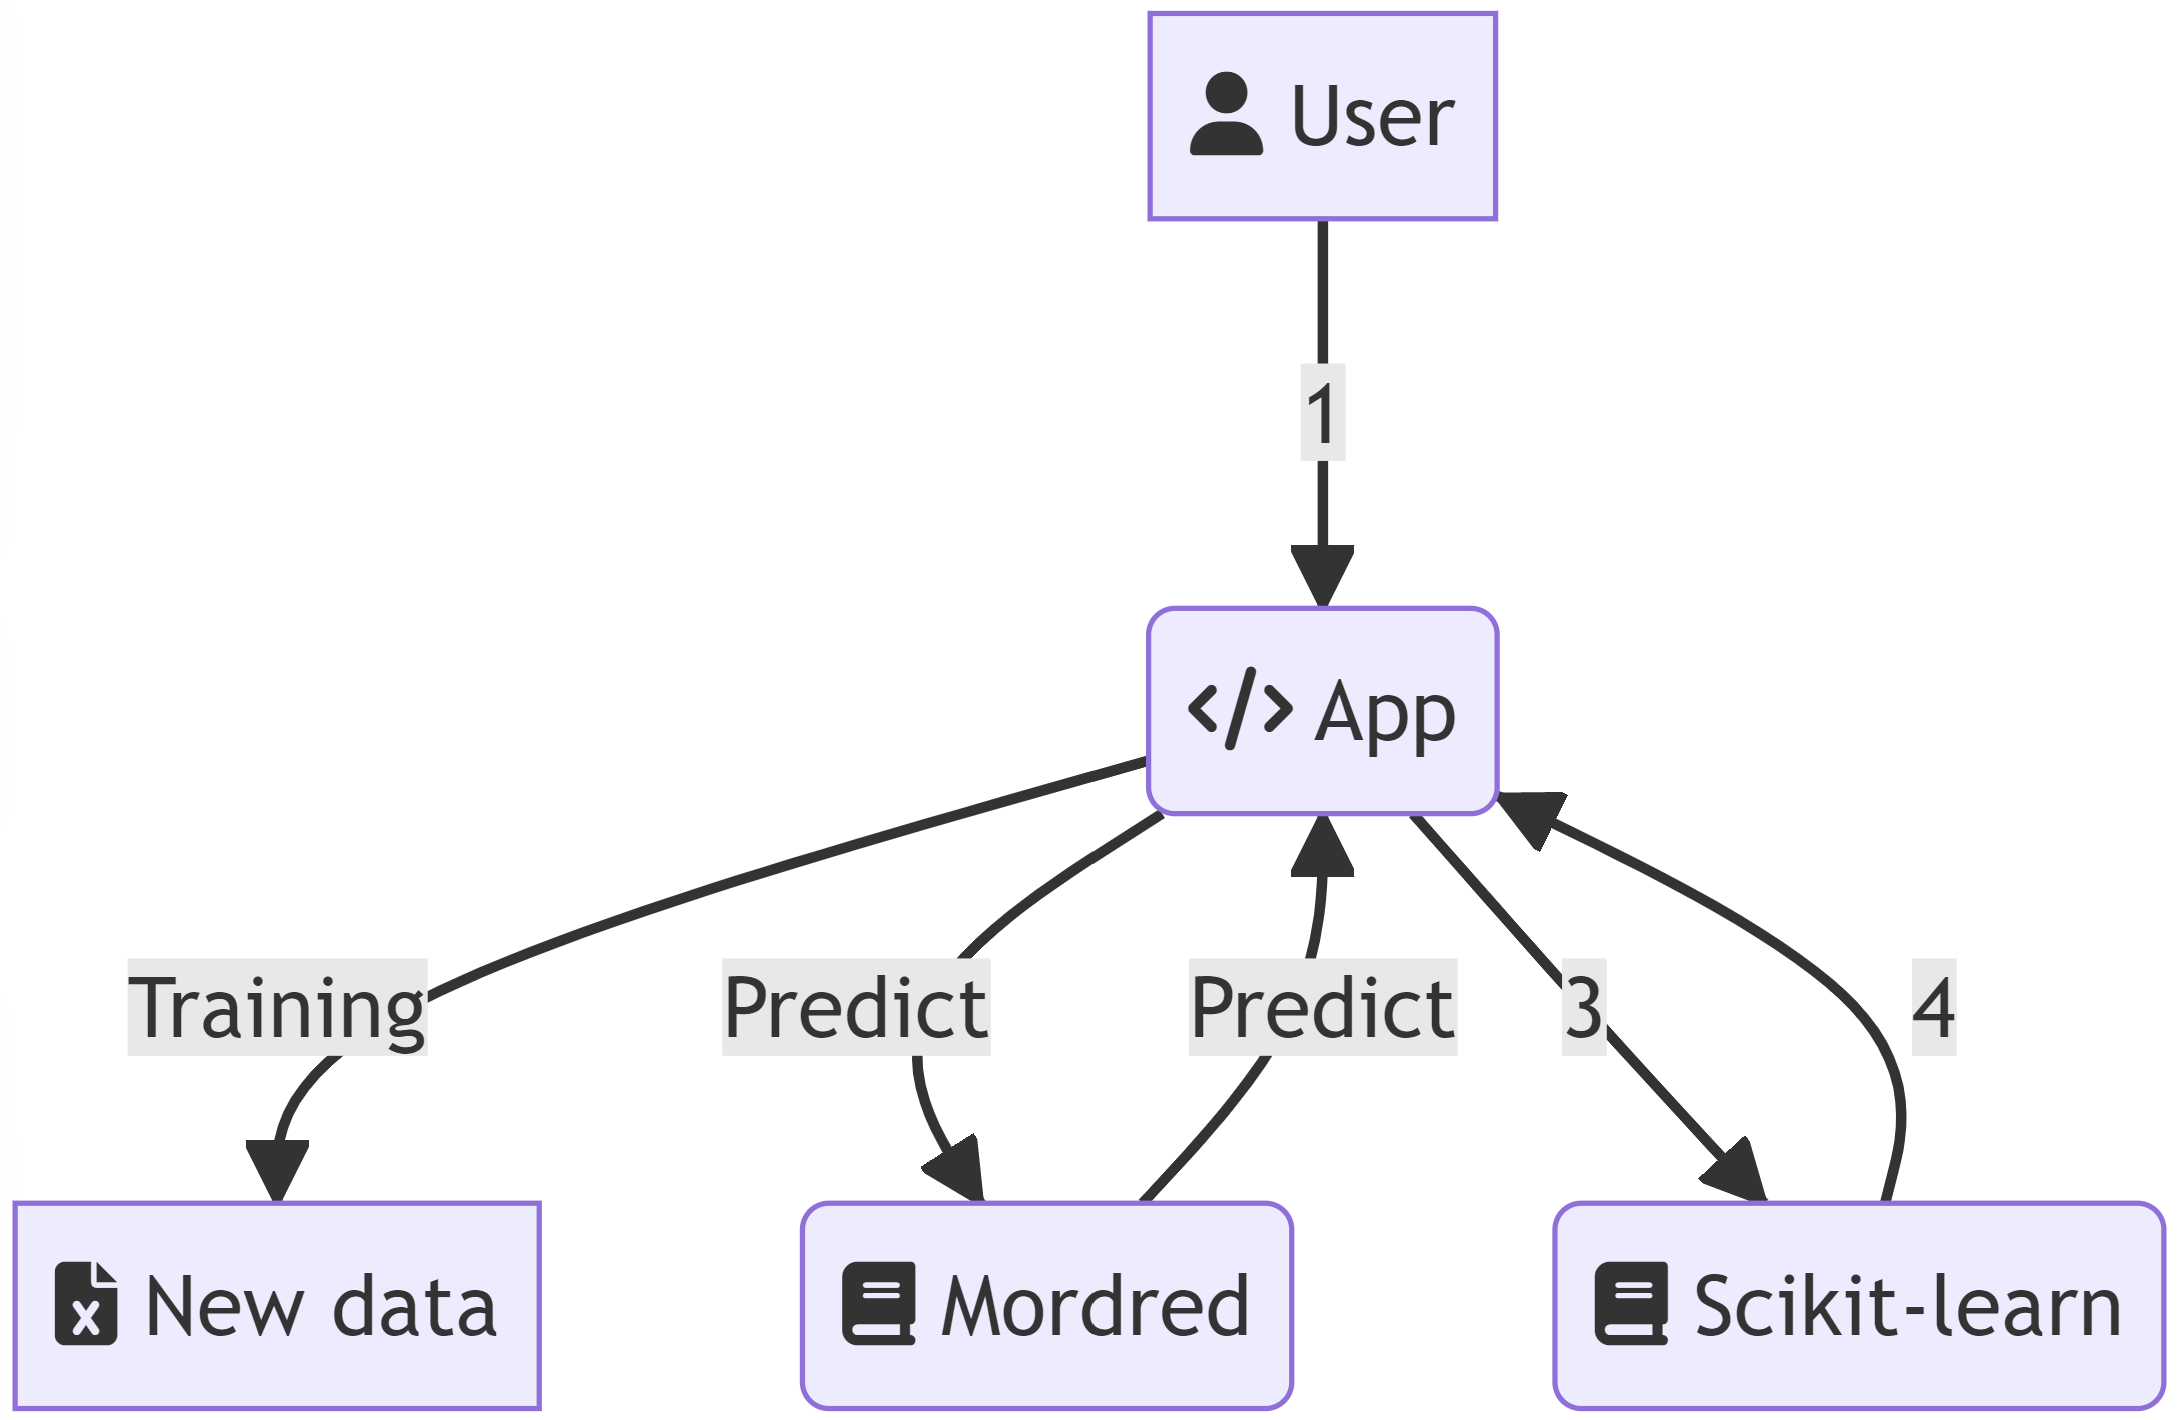
\includegraphics[width=100mm]{img/conception-ml-pipeline.png}
    \captionof{figure}{Activité de l'application de Machine Learning}
\end{center}

Le but est de fournir une seule application qui permet de tout faire et qui soit paramétrable à l'aide d'arguments.

% New page
\newpage
\subsection{Pipeline d'entraînement}
Si on rentre dans le détail de processus d'entraînement, il y a plusieurs étapes:
\begin{center}
    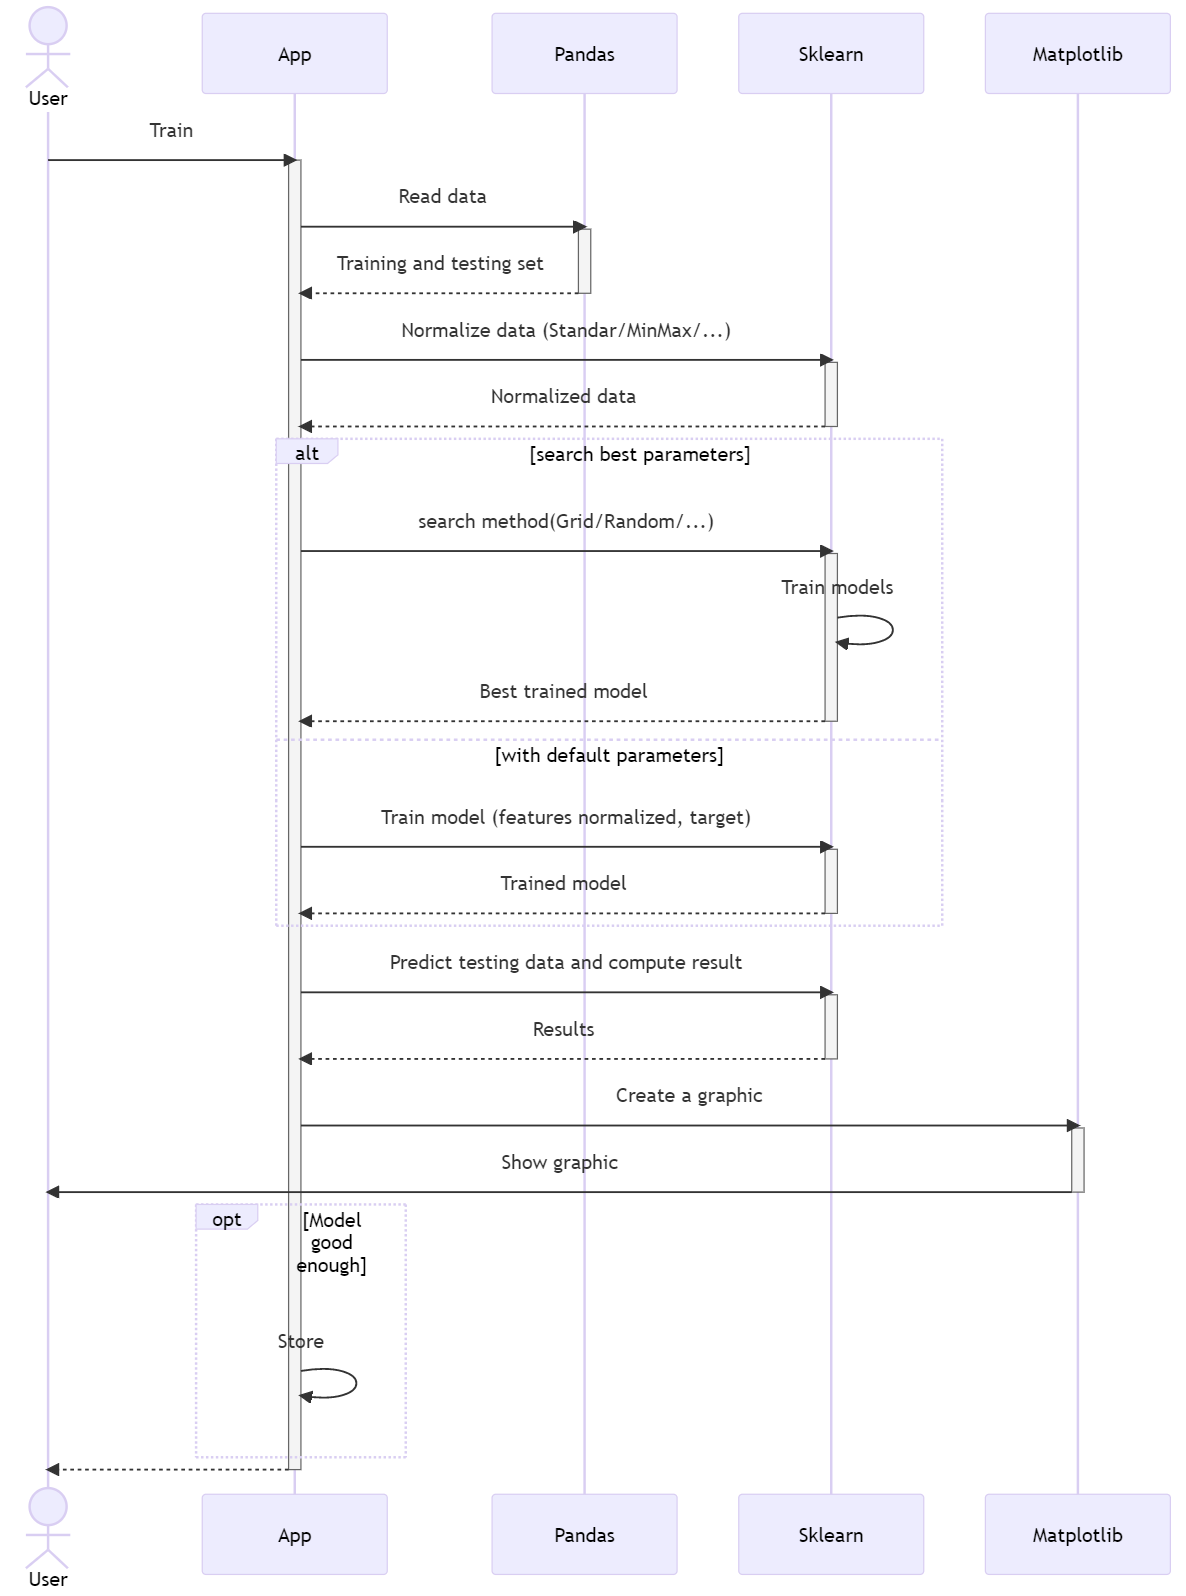
\includegraphics[width=140mm]{img/conception-ml-pipeline-training.png}
    \captionof{figure}{Pipeline de Machine Learning pour l'entraînement}
\end{center}

Le but est de pouvoir configurer chaque étape avec des paramètres lors du lancement du script.


\subsection{Sélection des features}
Pour sélectionner les bonnes features, il n'y a pas de méthode magique.
Ceci se fait par essaie-erreur en testant plusieurs combinaisons de features avec différents modèles et normalisation.
A cause du fait que le nombre de feature est important, il est difficile de les visualiser ou de les analyser.
Si les résultats sont plus mauvais qu'avec les donnnées de base, il faut essayer avec un mixte des données.
Si les modèles sont assez performants, ils sélectionnerons naturellement les bonnes features.
Si les meilleurs features ne sont que les features de base, ceci indique que les données rajoutées n'apportent rien d'utile à la prédiction.


%------------------------------------------------------------------------------
\section{Axe d'amélioration de l'\acrshort{ux}}
Si les résultats d'un modèle sont statisfaisant, il faudra ensuite le mettre à disposition de ChemTech pour qu'ils puissent l'utiliser.
Il y a 3 axes d'améliorations possible.

La premier est une version Desktop.
Je ne pense pas qu'il faut partir dans cette idée car l'utilisation est relativement simple et il y a le désanvatage de devoir l'installer.

La deuxième est un \acrfull{cli}.
Comme pour le version desktop, il y a le désanvantge de devoir l'installer, en revanche, ceci est beaucoup plus léger et cette solution est plus rapide à mettre en place.

La troisième est une version Web.
Cette solution n'a pas besoin d'être installée sur chaque ordinateur et l'application peut facilement être hébergé sur le serveur kubernetes de l'école.
Le désavantage est le temps de développement pour faire une vue et une \acrfull{api}.


